%-------------------------------------------------------------------------------
%   Haskellerのための圏論 - Kleisli-トリプル
%   Keichi
%   圏論の勉強成果の個人的なまとめ
%-------------------------------------------------------------------------------

%-------------------------------------------------------------------------------
\newpage
\section{Kleisliトリプル}

\subsection{定義}
Haskellで一般的に「モナド」と呼ばれているものは実は圏論のモナドとは
異なっていって、直接的に対応するのは圏論でKleisliトリプルとよばれている。

圏$C$上のKleisliトリプル(Kleisli-Triple)とは
\begin{itemize}
    \item 関数$T:Ob(C)\to Ob(C)$
    \item 射$\eta_A:\to T(A)$(各$A\in Ob(C)$)
    \item $(-)^*$: 射$f^*:T(A)\to T(B)$を各$f:A\to T(B)\in Ar(C)$についてつくる演算子
\end{itemize}
からなる3つ組(トリプル)$(T, \eta, (-)^*)$である。

\subsection{公理}
また、Kleisliトリプルは以下の条件を満たす:
\begin{itemize}
    \item $\eta_A^*=id_{T(A)}$
    \item $f:A\to T(B)$なら、$f^*\circ \eta_A=f$
    \item $f:A\to T(B)$なら、$g^*\circ f^*=(g^*\circ f)^*$
\end{itemize}

\begin{figure}[htbp]
    \centering
    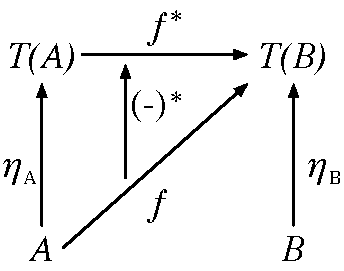
\includegraphics{diag_kleisli.pdf}
    \caption{Kleisliトリプル}
\end{figure}

\subsection{Haskellでの例}
HaskellのモナドはKleisliトリプルと対応する。型クラスMonadの定義は
\begin{lstlisting}
class Monad t where
    (>>=)   ::  t a -> (a -> t b) -> t b
    return  ::  a -> t a
\end{lstlisting}
であり、これはそれぞれ、
\begin{itemize}
    \item Monadのインスタンスのデータコンストラクタ(MaybeならJust)が関数$T$
    \item returnが$\eta$
    \item $(=<<)$が$(-)^*$
\end{itemize}
というように圏論のKleisliトリプルと対応している。
また、上記のKleisliトリプルの満たすべき条件は、以下のHaskellのモナド則に
それぞれ対応する。
\begin{lstlisting}
    (return x) >>= f    == f x
    m >>= return        ==  m
    (m >>= f) >>= g     ==  m >>= (\x -> f x >>= g)
\end{lstlisting}
